\chapter{Acquisition-System Design}
\section{Overview}
This section covers the development process including the hardware and firmware design of the audio acquisition system.
The goal of the acquisition system is to provide a flexible microphone recording infrastructure to easily aquiring audio signals from multiple microphones.


\subsection{Key Requirements}
% The main focus of the development is to design a professional looking, easy to use and eye-catching device for demonstration purposes.
% The project name \textit{Audio-Beamformer} has been chosen as it is easy to remember and has potential to be seen as a trademark.

The following key requirements have been set:
% \begin{itemize}
% 	\item Single power adapter or power cable (e.g. no need of labor power supplies)
% 	\item Easy to install (e.g. montage on a camera tripod)
% 	\item Intuitive to operate via state-of-the-art graphical user interface
% 	\item Multiple audio streaming sources such as Bluetooth and USB input devices
% 	\item Great scalability and flexibility of the hardware and software design
% \end{itemize}

\subsection{Key Decisions}



\newpage
\section{Hardware Design}

\begin{figure}[h]
	\centering
	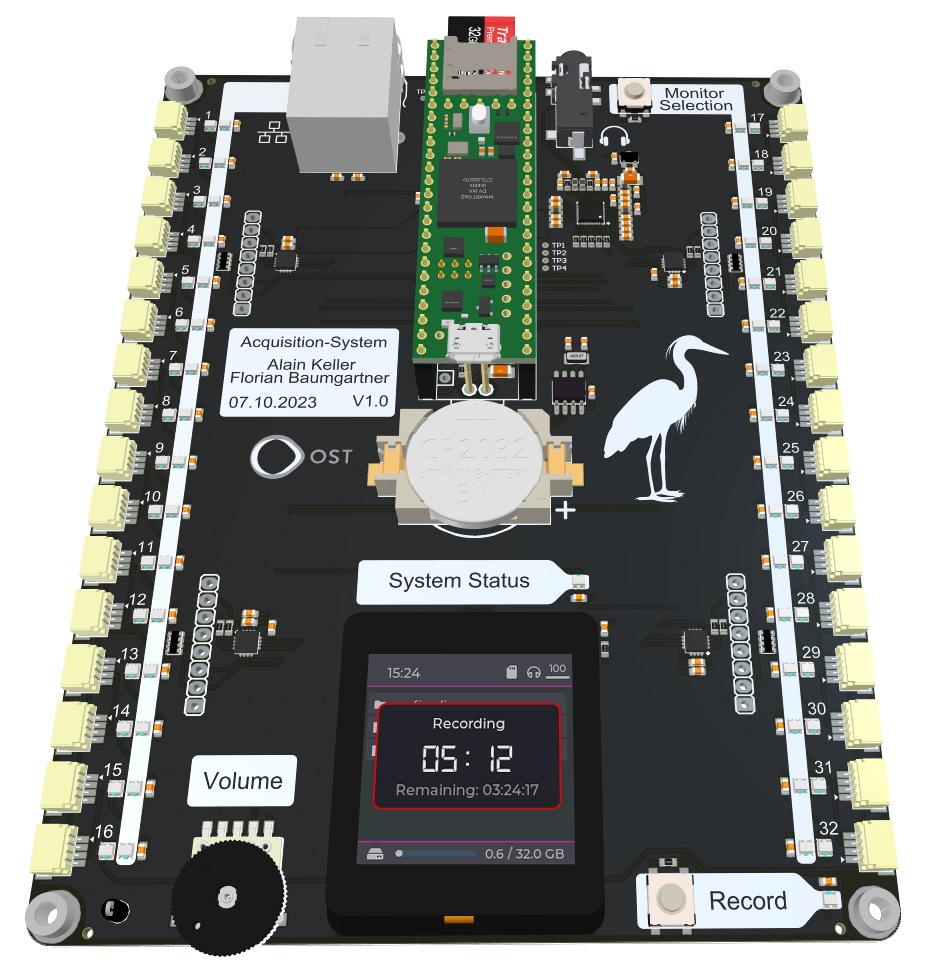
\includegraphics[width=1.0\textwidth]{images/4_design_acquisition_system/Acquisition_System_Front.png}
	\caption{Front view of the Acquisition System}
	\label{fig:acquisition_system_front}
\end{figure}


\subsection{Block Diagram}

\begin{figure}[h]
	\centering
	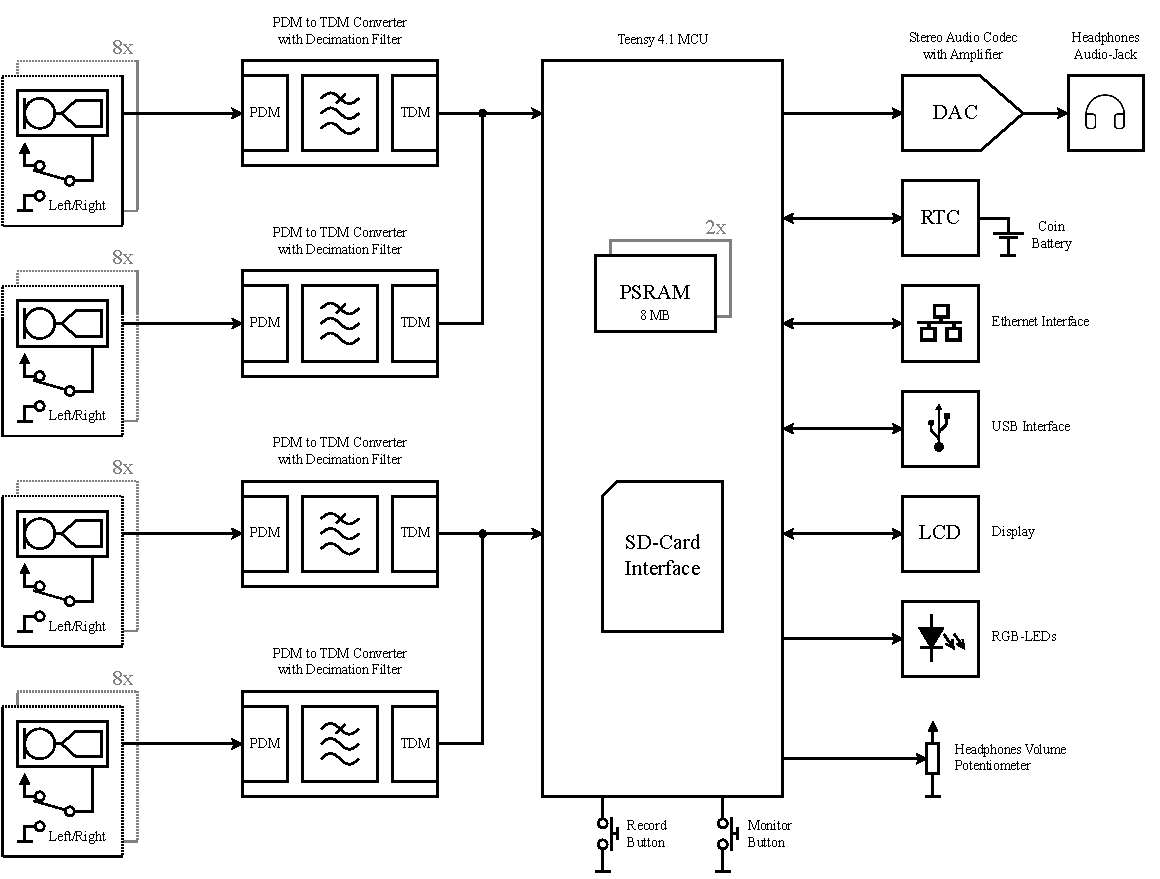
\includegraphics[width=1.0\textwidth]{images/4_design_acquisition_system/acquisition_system_design_block_diagram.pdf}
	\caption{System block diagram of acquisition system}
	\label{fig:acquisition_system_design_block_diagram}
\end{figure}

\subsection{Microcontroller Unit (MCU)}

%  TODO: Write about external PSRAM


\subsection{Audio Input}

\subsection{Audio Processing}

\subsection{Headphone Output}

To prelisten the individual audio channels, a headphone output is implemented.

% description of headphones jack
The headphone output is a standard 3.5mm stereo jack.



\newpage
\section{Firmware Design}
Blabla

\subsection{Graphical User Interface (GUI)}

\subsubsection{Light and Versatile Embedded Graphics Library (LVGL)}
LVGL (Light and Versatile Graphics Library) is a free and open-source graphics library, primarily used for creating embedded GUIs (Graphical User Interfaces).
It's designed to be lightweight, consuming minimal memory and processing power, which is essential in embedded systems where resources are limited.

The decision to use LVGL in conjunction with the NXP GuiGuider, a graphical design tool, enables a rich set of features and enables rapid development.
GuiGuider provides a user-friendly interface for designing GUIs, significantly simplifying the process of creating complex, visually appealing interfaces for embedded systems.
It also provides a code generator, which generates the necessary code to initialize and use the GUI in the firmware.

\subsection{GUI Pages}
The \acrshort{gui} is minimalisticly designed and straight forward to use.
The navigation between the main pages is done by swiping left or right on the touchscreen.
Next, the individual pages are described in detail.

\begin{minipage}{\linewidth}
	\begin{wrapfigure}{l}{4.5cm}
		\vspace{-0.6cm}
		
\includegraphics[width=4cm]{images/4_design_acquisition_system/gui/01_splash_screen.png}
		\centering
		\caption{Splash screen}
		\label{fig:acquisition_system_gui_splash_screen}
	\end{wrapfigure}
	\subsubsection{Splash Screen}
	When the device is powered on, the splash screen is displayed until the boot process is finished.
	On average this takes about 5 seconds.
\end{minipage}
\vspace{2.2cm}

\begin{minipage}{\linewidth}
	\begin{wrapfigure}{l}{4.5cm}
		\vspace{-0.6cm}
		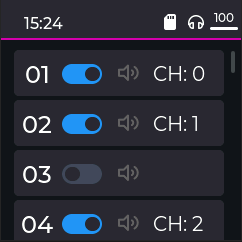
\includegraphics[width=4cm]{images/4_design_acquisition_system/gui/03_channel_settings.png}
		\centering
		\caption{Channel Settings}
		\label{fig:acquisition_system_gui_channel_settings}
	\end{wrapfigure}
	\subsubsection{Channel Settings}
	After the boot process is finished, the channel settings page is displayed.
	In the header bar located at the top of the page, the current time, \acrshort{usb} interface status, SD-Card status and headphones volume are displayed.
	A list of all 32 microphone inputs is shown in the center of the page.
	Each input channel can be enabled or disabled by clicking on the corresponding switch.
	When an input is enabled, its associated channel number of the WAV file is displayed.
	A speaker symbol shows if the channel is currently routed to the headphones monitor output (green means active, grey means inactive).
\end{minipage}
\vspace{0.0cm}

\begin{minipage}{\linewidth}
	\begin{wrapfigure}{l}{4.5cm}
		\vspace{-0.6cm}
		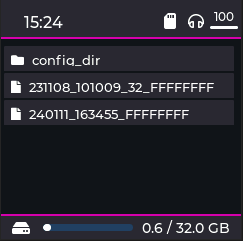
\includegraphics[width=4cm]{images/4_design_acquisition_system/gui/02_file_browser.png}
		\centering
		\caption{File Browser}
		\label{fig:acquisition_system_gui_file_browser}
	\end{wrapfigure}
	\subsubsection{File Browser}
	The file browser shows all files and folders located on the SD-Card.
	On the bottom of the page, a status bar indicates the current free and used space of the SD-Card.
	Due to the limited amount of memory, only the first 100 files and folders are displayed.
	This is however sufficient for most use cases.
\end{minipage}
\vspace{1.8cm}

\begin{minipage}{\linewidth}
	\begin{wrapfigure}{l}{4.5cm}
		\vspace{-0.6cm}
		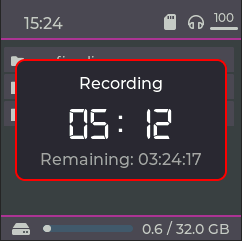
\includegraphics[width=4cm]{images/4_design_acquisition_system/gui/04_recording.png}
		\centering
		\caption{Recording}
		\label{fig:acquisition_system_gui_recording}
	\end{wrapfigure}
	\subsubsection{Recording}
	When the record button is pressed, the recording begins and a panel overlay is displayed.
	In the centre of the panel, the current recording time is displayed in minutes and seconds.
	Below, the remaining recording time is shown.
	When the recording is stopped, the panel overlay disappears.
	While the device is recording, all \acrshort{ui} elements and the navigation are disabled.
\end{minipage}
\vspace{1.8cm}

\begin{minipage}{\linewidth}
	\begin{wrapfigure}{l}{4.5cm}
		\vspace{-0.6cm}
		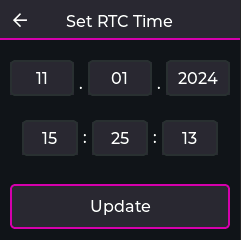
\includegraphics[width=4cm]{images/4_design_acquisition_system/gui/05_set_time.png}
		\centering
		\caption{Set RTC Time}
		\label{fig:acquisition_system_gui_set_time}
	\end{wrapfigure}
	\subsubsection{Set RTC Time}
	When the user clicks on the time in the header bar, the set time page is displayed.
	There the user can set the current time and date.
	After clicking on the \textit{Update} button, the new time is set and the page is closed.
	To abort the process, the user can click on the arrow in the header bar.
\end{minipage}
\vspace{1.8cm}



